\documentclass[12pt]{article}

\usepackage[margin=1in]{geometry}
\usepackage{tikz}
\usepackage{array}
\usepackage{amsmath}
\usepackage{amssymb}

\pagestyle{empty}

\begin{document}

% ==================================================
% Corner alignment markers
% ==================================================

\begin{tikzpicture}[remember picture, overlay]

% Each marker is 5 mm x 5 mm, outer corner 15 mm from the page edge
% on every side — anchored to the physical page, not the text area,
% so all four markers are symmetric and within any printer's safe zone.

% top-left
\fill[black]
  ([xshift=15mm, yshift=-20mm]current page.north west)
  rectangle
  ([xshift=20mm, yshift=-15mm]current page.north west);

% top-right
\fill[black]
  ([xshift=-20mm, yshift=-20mm]current page.north east)
  rectangle
  ([xshift=-15mm, yshift=-15mm]current page.north east);

% bottom-left
\fill[black]
  ([xshift=15mm, yshift=15mm]current page.south west)
  rectangle
  ([xshift=20mm, yshift=20mm]current page.south west);

% bottom-right
\fill[black]
  ([xshift=-20mm, yshift=15mm]current page.south east)
  rectangle
  ([xshift=-15mm, yshift=20mm]current page.south east);

\end{tikzpicture}

\vspace*{1cm}

\begin{center}
    {\Large OMR Test Template (Mixed Choices)}
\end{center}

\vspace{1cm}

% ==================================================
% Question 1 — 4 choices
% ==================================================

\noindent
Question 1 \hfill \textit{(4 choices)}

\vspace{0.3cm}

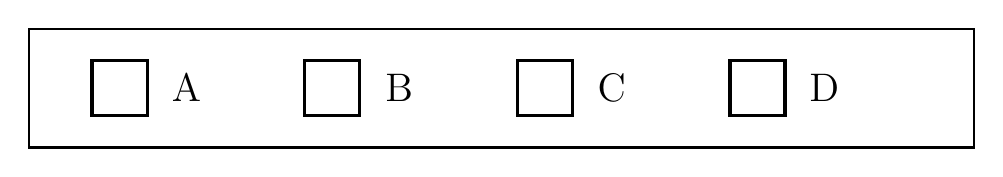
\begin{tikzpicture}
\draw[line width=1pt] (0,0) rectangle (12,1.5);

\draw[line width=1.2pt] (0.8,0.4) rectangle (1.5,1.1);
\node at (2.0,0.75) {\Large A};

\draw[line width=1.2pt] (3.5,0.4) rectangle (4.2,1.1);
\node at (4.7,0.75) {\Large B};

\draw[line width=1.2pt] (6.2,0.4) rectangle (6.9,1.1);
\node at (7.4,0.75) {\Large C};

\draw[line width=1.2pt] (8.9,0.4) rectangle (9.6,1.1);
\node at (10.1,0.75) {\Large D};
\end{tikzpicture}

\vspace{1cm}

% ==================================================
% Question 2 — 2 choices (B ticked as example)
% ==================================================

\noindent
Question 2 \hfill \textit{(2 choices)}

\vspace{0.3cm}

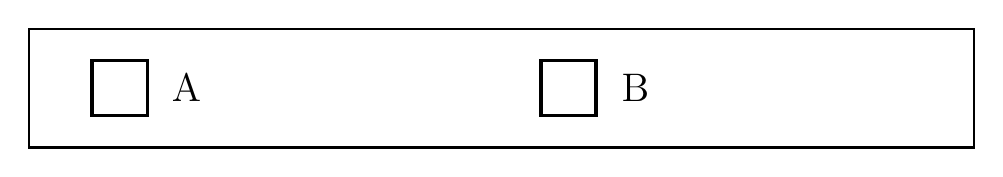
\begin{tikzpicture}
\draw[line width=1pt] (0,0) rectangle (12,1.5);

\draw[line width=1.2pt] (0.8,0.4) rectangle (1.5,1.1);
\node at (2.0,0.75) {\Large A};

\draw[line width=1.2pt] (6.5,0.4) rectangle (7.2,1.1);
\node at (7.7,0.75) {\Large B};
\end{tikzpicture}

\vspace{1cm}

% ==================================================
% Question 3 — 6 choices
% ==================================================

\noindent
Question 3 \hfill \textit{(6 choices)}

\vspace{0.3cm}

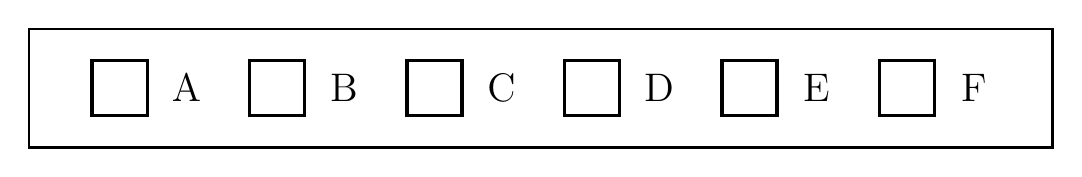
\begin{tikzpicture}
\draw[line width=1pt] (0,0) rectangle (13,1.5);

\draw[line width=1.2pt] (0.8,0.4) rectangle (1.5,1.1);
\node at (2.0,0.75) {\Large A};

\draw[line width=1.2pt] (2.8,0.4) rectangle (3.5,1.1);
\node at (4.0,0.75) {\Large B};

\draw[line width=1.2pt] (4.8,0.4) rectangle (5.5,1.1);
\node at (6.0,0.75) {\Large C};

\draw[line width=1.2pt] (6.8,0.4) rectangle (7.5,1.1);
\node at (8.0,0.75) {\Large D};

\draw[line width=1.2pt] (8.8,0.4) rectangle (9.5,1.1);
\node at (10.0,0.75) {\Large E};

\draw[line width=1.2pt] (10.8,0.4) rectangle (11.5,1.1);
\node at (12.0,0.75) {\Large F};
\end{tikzpicture}

\vspace{1cm}

% ==================================================
% Question 4 — 4 choices
% ==================================================

\noindent
Question 4 \hfill \textit{(4 choices)}

\vspace{0.3cm}

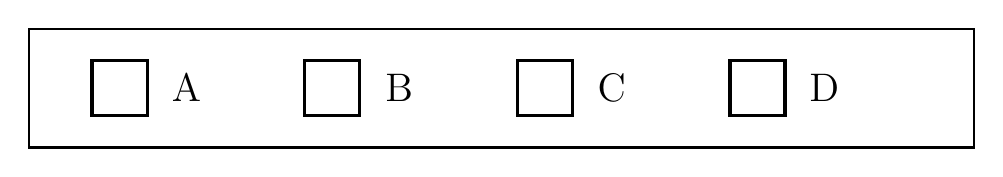
\begin{tikzpicture}
\draw[line width=1pt] (0,0) rectangle (12,1.5);

\draw[line width=1.2pt] (0.8,0.4) rectangle (1.5,1.1);
\node at (2.0,0.75) {\Large A};

\draw[line width=1.2pt] (3.5,0.4) rectangle (4.2,1.1);
\node at (4.7,0.75) {\Large B};

\draw[line width=1.2pt] (6.2,0.4) rectangle (6.9,1.1);
\node at (7.4,0.75) {\Large C};

\draw[line width=1.2pt] (8.9,0.4) rectangle (9.6,1.1);
\node at (10.1,0.75) {\Large D};
\end{tikzpicture}

\vspace{1cm}

% ==================================================
% Question 5 — 6 choices
% ==================================================

\noindent
Question 5 \hfill \textit{(6 choices)}

\vspace{0.3cm}

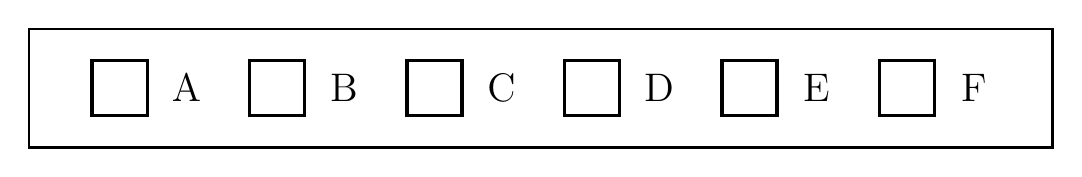
\begin{tikzpicture}
\draw[line width=1pt] (0,0) rectangle (13,1.5);

\draw[line width=1.2pt] (0.8,0.4) rectangle (1.5,1.1);
\node at (2.0,0.75) {\Large A};

\draw[line width=1.2pt] (2.8,0.4) rectangle (3.5,1.1);
\node at (4.0,0.75) {\Large B};

\draw[line width=1.2pt] (4.8,0.4) rectangle (5.5,1.1);
\node at (6.0,0.75) {\Large C};

\draw[line width=1.2pt] (6.8,0.4) rectangle (7.5,1.1);
\node at (8.0,0.75) {\Large D};

\draw[line width=1.2pt] (8.8,0.4) rectangle (9.5,1.1);
\node at (10.0,0.75) {\Large E};

\draw[line width=1.2pt] (10.8,0.4) rectangle (11.5,1.1);
\node at (12.0,0.75) {\Large F};
\end{tikzpicture}

\end{document}

